%!TEX root = ../main.tex

\chapter{Introduction}
\label{chp:intro}

The term \ac{NTNs} denotes a category of networks where at least one link is routed via an aerial or space-borne vehicle such as \ac{HAPs}, \ac{UAVs} or telecommunication satellites.

\section{The focus on non-terrestrial networks}
The Third Generation Partnership Project \footnote{\href{https://www.3gpp.org}{\texttt{3gpp.org}}} (3GPP), the standardization body developing protocols for mobile communication networks, recently put a great emphasis on the importance of the integration of different access technologies along with the existing terrestrial mobile telecommunication infrastructure \cite{3gpp-tr-21.917}.

The envisioned future for mobile communications, starting with the already established 5G \ac{NR} and expanding with the new sixth-generation cellular networks (6G), foresees the integration of a non-terrestrial component. The latest \ac{3GPP} releases (Rel. 17 and Rel. 18) require 5G and 6G networks to be able to provide non-terrestrial satellite access complementing the already existing terrestrial access technologies \cite{overview-rel-17-18-saad} \cite{5g-nr-communication-geo-leo-maattanen}.

\section{Limitations of terrestrial networks}
The following paragraphs present a few scenarios where terrestrial networks have some limitations, and \ac{NTNs} can be used to provide connectivity.

\subsection{Remote places}
While \ac{TN} make the well-established foundation of today’s mobile communication infrastructure, their own nature poses some intrinsic limitations to their deployment in certain scenarios, especially in rural and remote areas. Conditions such as harsh terrain and geographical impediments act as natural barriers to the deployment of terrestrial infrastructure. Moreover, ground infrastructure requires the presence of an already established reliable power grid, driving up the costs that telecommunication companies would have to sustain.
The population density is often low in remote and rural places, so the already high infrastructure cost will hardly pay for itself, making this kind of market even more unattractive to private investors and further limiting the possibility for the people living there to access a resource which is becoming increasingly more important.

As studied and documented in \cite{6g-challenge-opportunity-base-pyramid}, the issue of an inadequate broadband coverage in rural regions is an enormous challenge, but also a great opportunity to kick-start the economy of currently underdeveloped countries, promoting a more fair access to the internet and alleviating the problem of digital divide between different parts of the world.

\subsection{Redundancy}
Another limitation of the current terrestrial infrastructure is the lack of redundancy and robustness against natural disasters. Extreme events such as earthquakes, fires and floods, but also deliberate behaviors such as targeted attacks by terrorist organizations and sabotages can disrupt the connectivity even for a long period of time, causing significant economical damage and hindering the already difficult rescue efforts, potentially leading to loss of lives.

The simple installation of a greater number of base stations is not a viable solution because they all share the same weaknesses.

In this scenario, \ac{NTNs} can act as redundant access methodology to decrease downtimes of terrestrial infrastructure, provide emergency communication services and also additional capacity when required. 

\subsection{Long distances and sensors}
Remote equipment, offshore plants and distribution grids will also benefit from the research carried out in this field, since providing terrestrial connectivity in those scenarios is a challenging task. The installation of an underwater optical fiber link to serve a single endpoint, such as an offshore power plant in the ocean, would bear a disproportional cost compared to the functions required, and maintenance would be another challenging and expensive task. 
The deployment of a non-terrestrial network would provide connectivity on a global scale, therefore allowing internet access in isolated places without the need for a dedicated connection.

Consider now the problem of connecting of a number of sensors placed in a large area. When distances are large, solutions may either be the densification of radio stations or the use of a lower frequency in order to have a less severe propagation loss. However, those approaches have their downsides and are not always feasible. In this case, the large coverage area of \ac{NTNs} will undoubtedly be useful to provide internet connection \cite{performance-ntn-support-iot-wang}.

\paragraph{} Other scenarios where \ac{NTNs} can become useful in overcoming the limitation of their terrestrial counterpart are well described in \cite{ntn-6g-era-challenges-giordani} and \cite{potential-multilayered-nierarchical-ntn-wang}.

\section{Satellite types}
Satellites are divided in three different categories depending on their orbiting altitude: \ac{GEO}, \ac{MEO} \ac{LEO} satellites. Each one has its own characteristics, as briefly described below.

\subsection{GEO satellites}
orbiting at 35.786Km, \ac{GEO} satellites appear stationary since their orbiting period is the same as the Earth rotation period. This vastly simplifies the tracking for the ground equipment, since once the position of the \ac{UE} is known, the relative position of the satellite is known, too.
    
Since \ac{GEO} satellites are geostationary, continuous coverage to a designated area can be provided using as little as a single satellite, while the use of non-\ac{GEO} satellites would require the deployment of a constellation, which is both more complex and more expensive.

Their higher altitude creates a large cell footprint, larger than both \ac{MEO} and \ac{LEO}, so the overall cost to provide coverage to the same area is lower.

The disadvantages of \ac{GEO} satellites are mainly linked to the large distance with the \ac{UE}: the transmission power and the antenna gain have to be higher to account for the greater propagation losses, and the propagation delay of the signal travelling at the speed of light is about 120ms, so if the \ac{UE} sends a request to a server at time zero through a \ac{GEO} link, the best-case delay will be of half a second without considering any protocol-related delay.

In addition to the positive aspects previously discussed, the larger cell footprint also means that a single satellite will be serving a massive number of users, so the total available capacity will have to be shared between a bigger number of actors, and the throughput experienced by each one of them will be reduced. 
Moreover, the high number of users leads to a large rate of initial access  requests, with the possibility of channel saturation as described in \cite{3gpp-tr-38.811}.

\subsection{LEO satellites}
Orbiting below the altitude of 2.000Km, \ac{LEO} satellites are the most promising solution in the realm of \ac{NTNs} for a number of reasons hereby discussed.
    
The lower altitude entails a shorter propagation delay, and the smaller coverage area of each satellite means that the total number of users that need to be served is smaller. 

The cost per satellite is significantly smaller than \ac{GEO} and \ac{MEO} satellites. However, given that they are not geostationary, a large constellation is needed to provide a continuous service, driving up the deployment costs significantly. As an example of those constellations, Fig. \ref{fig:starlink_constellation} depicts the \ac{LEO} satellites employed by Starlink\footnote{Starlink is a satellite internet constellation operated by Starlink Services, LLC, a wholly-owned subsidiary of American aerospace company SpaceX.}, with 4.808 units in service at the time of writing\footnote{Source: \href{https://satellitemap.space/}{\texttt{satellitemap.space}}}.

\begin{figure}[ht]
    \centering
    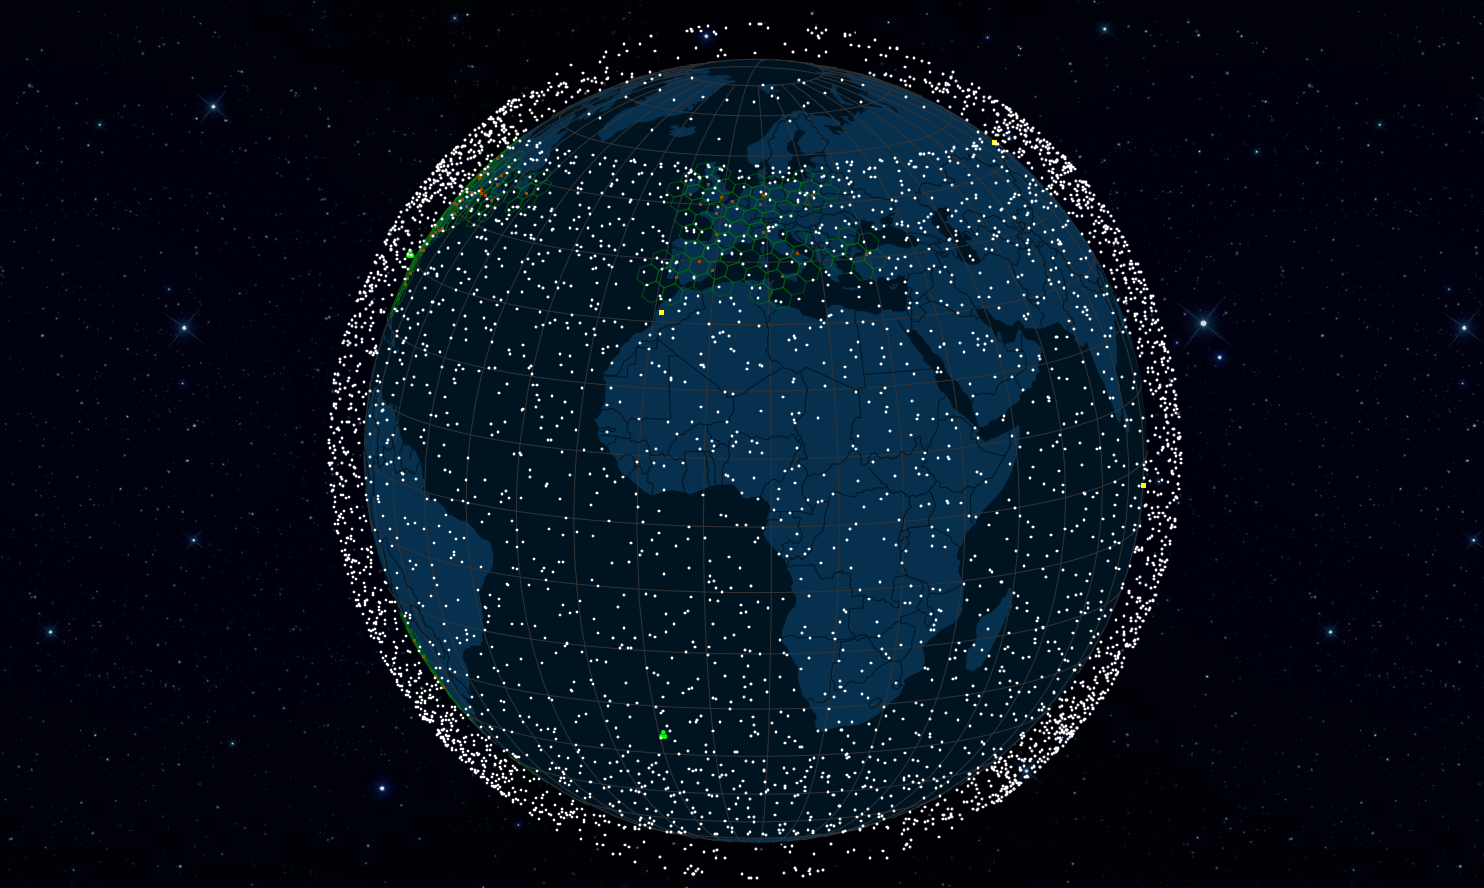
\includegraphics[width=0.7\textwidth]{res/starlink-constellation.png}
    \caption{Starlink constellation as July 2024. Source: \href{https://satellitemap.space/}{\texttt{satellitemap.space}}}
    \label{fig:starlink_constellation}
\end{figure}

The smaller altitude at which \ac{LEO} satellites orbit enables the use of higher frequency bands, since the experienced path loss is smaller compared to \ac{GEO} satellites. This in turn allows for higher throughput, as detailed in \cite{satellite-communication-mmwave-giordani}

The aforementioned solutions are not to be considered mutually exclusive. In fact, the multitude of possibilities that their combinations offer open to the study of various different scenarios, as detailed in \cite{potential-multilayered-nierarchical-ntn-wang}

\subsection{Current solutions}
Current solutions for non-terrestrial communication do exist, but they mostly rely on telecommunications satellites placed in the \ac{GEO}, at a height of 35.786 km. The distance that the signal has to travel offering limited throughput and large delays. While \ac{LEO} constellations (400 km to 2.000 km) have proven to be a valid alternative, providing higher throughput and lower latency \cite{main-features-5g-nr-ntn-yun}, they have the drawback of an increased Doppler shift due to their high speed relative to ground \cite{satellite-communication-mmwave-giordani}, and there is still no international standard with regard to the communication protocols to use. 

\paragraph{}
This scenario led \ac{3GPP} to identify some work to be done to integrate \ac{NTN} in cellular standards, calling for long-term research in this field \cite{satellite-communication-mmwave-giordani}. This work will mainly focus on the 

\paragraph{}\todo{move this to state of the art} Focusing on the \ac{MAC} sublayer, the large propagation delay of satellite links affects different aspects, making the actual implementation not suited for a \ac{NTN} scenario. In the \ac{HARQ} protocol, the retransmission timeout is likely to expire before a single \ac{RTT}, leading to unnecessary retransmissions. Moreover, the limit on the maximum number of concurrent \ac{HARQ} processes leads to a stop-and-wait behaviour, which may increase the energy consumption \cite{3gpp-tr-38.811}. On the other hand, it has been noted that disabling \ac{HARQ} would lead to an even worse performance penalty, therefore requiring a redesign for \ac{NTN} \cite{5g-beyond-5g-ntn-trends-vanellicoralli}. Another 5G \ac{NR} protocol which is negatively impacted in \ac{NTN} is the initial access, since users at the center of the cell face a smaller propagation delay with respect to users at the cell edge \cite{5g-beyond-5g-ntn-trends-vanellicoralli} \cite{applying-nr-technologies-in-ntn-lee}. As a result, preambles of \ac{UE}s placed near the cell edge may reach the satellite when the \ac{RACH} opportunity has already expired, which may lead to collisions. During the initial access phase, \ac{UE}s are not aware of their propagation delay, and the high mobility of \ac{gNB}s on \ac{LEO} satellites causes a non-negligible Doppler shift. Those factors vary with the relative position and speed between the \ac{UE} and the \ac{gNB}, and the protocols for initial access must be modified in \ac{NTN} to account for them \cite{ntn-from-5g-6g-hassan}. 
\paragraph{}
It is clear that the future of mobile networks envisioned by \ac{3GPP} embraces \ac{NTN}s, and considerable work has to be done. Research will bear a high impact towards a more connected, equal opportunity world. 

\section{Currrent state of the art}
\todo{types of payloads: regenerative, and transparent or bent pipe}